\documentclass[a4paper,11pt]{article}

\usepackage{float}
\usepackage{graphicx}
\setlength{\oddsidemargin}{0in}
\setlength{\evensidemargin}{0in}
\setlength{\textwidth}{160mm}
\setlength{\topmargin}{-15mm}
\setlength{\textheight}{240mm}
\graphicspath{./Diagrams}

\begin{document}
\section{Results and Conclusions}

\subsection{Comparing methods}
For the results in hybrid and multi-objective algorithms past the medium difficulty, both algorithms failed every single attempt that was made, therefore they will not be covered.
\subsubsection{Comparing Hybrid and Multi-objective 4x4}

\begin{figure}[h]
	\centering
	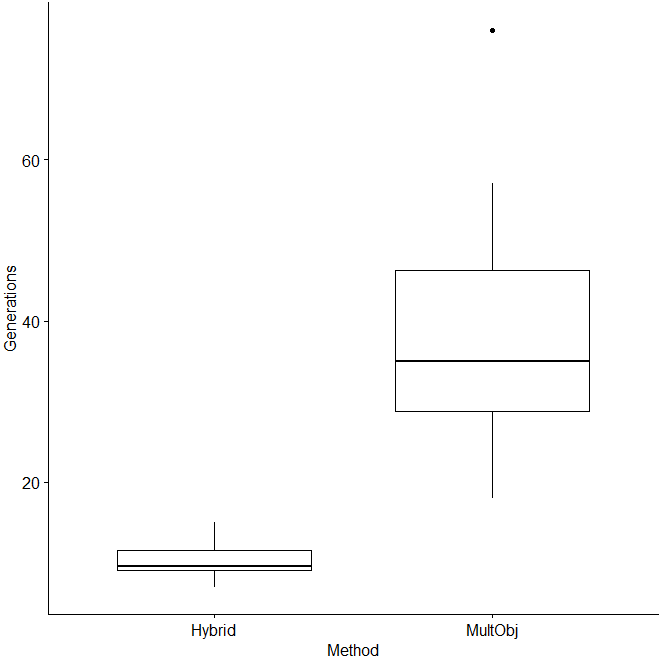
\includegraphics[height=10cm,width=10cm]{./Diagrams/barChartComparing4x4}
	\caption{Chart comparing generations on 4x4 sudokus}
\end{figure}

When looking at the two algorithms, looking at the chart and the results in general, the hybrid algorithm performs better, has less variance, and holds no outliers when it comes to generations. Whilst it is better when looking at these statistics, it is also worth mentioning that the scope of the chart, is rather zoomed in and the multi-objective solver equally performs quite well. This makes sense since the repair method used removes a lot of uncertainty due to its ability to remove values it knows are wrong. On the other hand since, the multi-objective solver does not have a clear set of rules which it follows, especially working on the 4x4 creates a larger amount of guess work for the solver. The IQR and median of the hybrid method are also lower, which builds on the idea, that for the 4x4 puzzles, the hybrid can reel in and control the randomness of the mutation. Doing a Wilcoxon test to compare the two solvers gave a p value of 0.0001766 and a w of 0, from which we can interpret that the two sets of data are very different from each other. Which shows that at least in terms of generations, that the hybrid algorithm is a more effective algorithm than the multi-objective solver.
\begin{figure}[h]
	\centering
	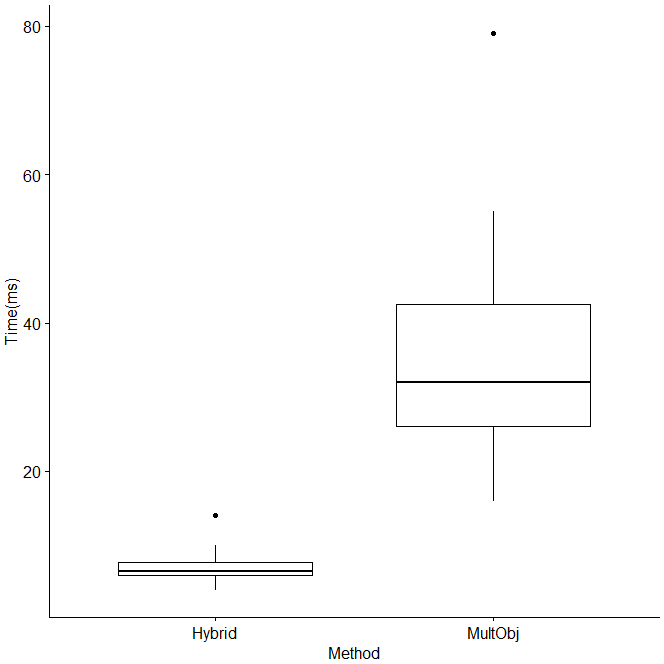
\includegraphics[height=10cm,width=10cm]{./Diagrams/barChart4x4Time}
	\caption{Chart comparing runtime on 4x4 sudokus}
\end{figure}
The runtime of the algorithms futher supports this conclusion, with a similar chart state to the generation chart. It is also worth noting that in the 4x4 puzzles neither algorithm failed to complete a single puzzle.

\subsubsection{Comparing Hybrid and Multi-objective 9x9 easy}
Results for 9x9 easy puzzles
\begin{figure}[h]
	\centering
	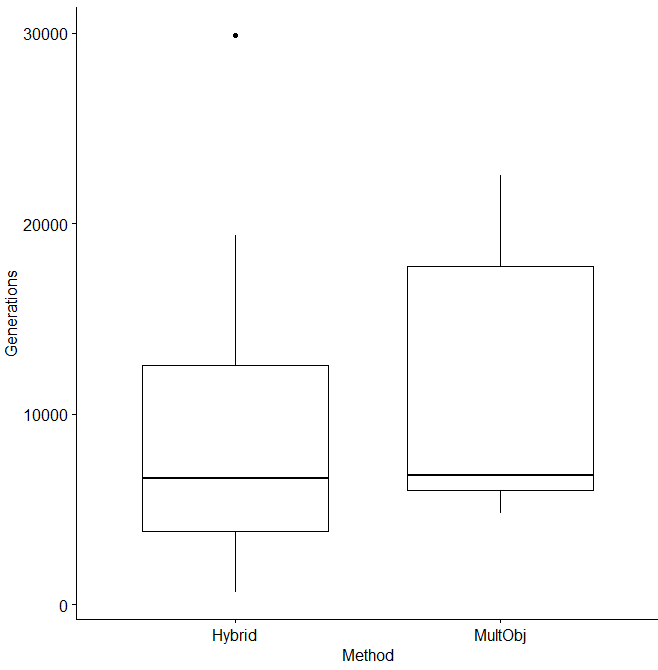
\includegraphics[height=10cm,width=10cm]{./Diagrams/barChartComparing9x9Easy}
	\caption{Chart comparing generations on easy 9x9 sudokus}
\end{figure}
By looking at the graphs alone, it could once again be concluded, that in general hybrid is a more efficient algorithm, however it has lost its stability as an algorithm, and has the same median as the multi-objective algorithm. Furthermore the hybrid algorithm also failed to complete puzzles 64 times out of the 300 runs over all the easy 9x9s. Whereas the multi-objective did not fail a single puzzle, has most of its results close to the hybrid results values. Looking at the Wilcoxon test results, the p value was 0.5205 with a w of 41, meaning the two are quite similar. However if the failed results were included in the data here, the multi-objective would have a smaller range, median and a smaller IQR.
\begin{figure}[h]
	\centering
	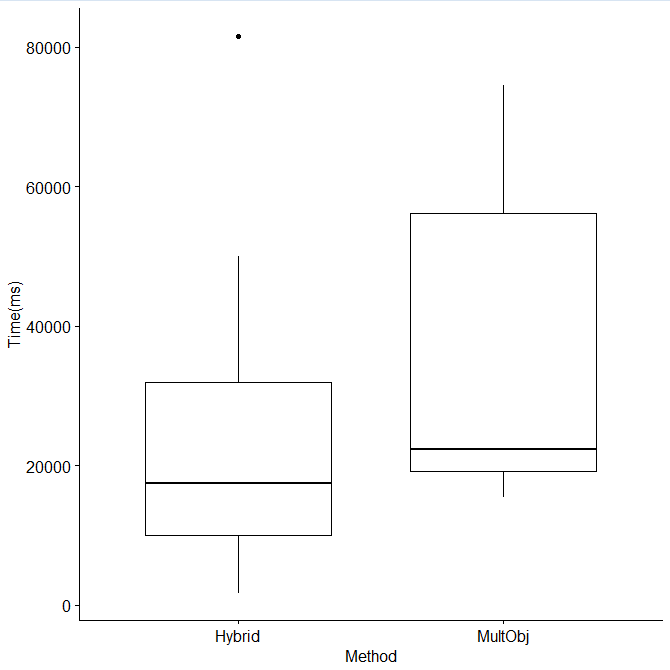
\includegraphics[height=10cm,width=10cm]{./Diagrams/barChart9x9EasyTime}
	\caption{Chart comparing runtime on easy 9x9 sudokus}
\end{figure}
The runtime excluding the failed values show that the hybrid method is generally faster but if the failed values were added, the averages would once again switch up. In the case of easy 9x9 sudokus, it seems multi-objective is a better option due to its failure rate of 0, which is worth the potential efficiency lost.
\subsubsection{Comparing Hybrid and Multi-objective 9x9 Medium}

Due to both solvers failed to complete most of the puzzles the data for this sections, is hard to map the data out in a way that displays any meaningful insight, so as an alternative the only comparison that can be made by this set is the runtime.
\begin{figure}[h]
	\centering
	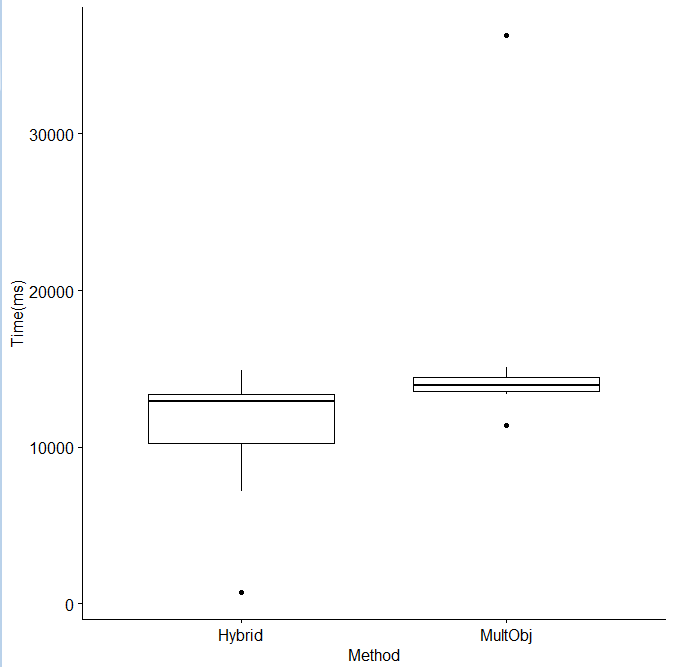
\includegraphics[height=10cm,width=10cm]{./Diagrams/barChartTime9x9Medium}
	\caption{Chart comparing runtime on medium 9x9 sudokus}
\end{figure}
Looking at the runtime, the hybrid algorithm seems to be faster on average, however it has a larger range in runtimes, once again shows the instability of the hybrid method. It is also worth noting that of the puzzles that were solved, the average number of generations for the hybrid methods was a lot lower than the average for the multi-objective algorithm.
\subsection{Conclusion for experiment 1}
In summary looking at the questions being asked in experiment 1 in section 2.1. For the question of which algorithm is more efficient, overall the hybrid algorithm tends to find an answer faster, however with an increase in size and difficulty, the chances of the hybrid algorithm getting stuck and not giving any answer, raises significantly higher than the multi-objective algorithm, which whilst having slower execution and using more generations, has a better chance of finding an answer, rather than getting stuck. The hybrid algorithms tendency to get stuck, could originate from its greedy repair algorithm, which only repairs, what appears to be the best option at the time, with no forward thinking being applied. The most consistent method out of the two seems to be the multi-objective solver, which has generally had a smaller IQR and range than the hybrid algorithm, furthermore the algorithm also seems to be able to find the correct answer more consistently than the hybrid algorithm.  


\subsection{Comparing difficulties}
Due to the insufficient data produced by the algorithms, it would be hard to make any conclusions about the different difficulties, and therefore also hard to comment on experiment 2 and the questions brought up in it. However if we look at how gradually both algorithms failed more with an increase of size, space and difficulty, so there is a high chance that these relationships exist and are just linked to the number empty squares in the starting state of the puzzle.

\end{document}